\documentclass{article}[10pt]
\usepackage{titling}
\setlength{\droptitle}{-10em}
\usepackage[margin=1in]{geometry}
\usepackage{amssymb}
\usepackage{epsfig}
\usepackage{subfigure}
\usepackage{graphicx}
\usepackage{wrapfig}
\usepackage{setspace}
\usepackage{textcomp}
\usepackage{cite}
\usepackage{float}
\usepackage{csquotes}
\usepackage{graphicx}
\makeatletter
\makeatother

\expandafter\let\csname equation*\endcsname\relax
\expandafter\let\csname endequation*\endcsname\relax
\usepackage{amsmath}
\newcommand{\agt}{\mathrel{\raise.3ex\hbox{$>$\kern-.75em\lower1ex\hbox{$\sim$}}}}
\begin{document}

\title{\emph{Frankenstein} and the horrors of competitive exclusion}


\author{N. J. Dominy \& J. D. Yeakel}

\date{}
% \begin{abstract}
%
%
% \end{abstract}


\maketitle
\vspace{-1.5cm}
Bicentennial celebration of the inception of Frankenstein motivates the present comment on Victor Frankenstein and his fateful decision to destroy an unfinished female creature. 
The act was impulsive (caused by a``\emph{sensation of madness}"), but it was preceded with agonized reasoning that would be familiar to any contemporary ecologist or evolutionary biologist. 
Here we present a formal treatment of this reasoning. 
Our findings suggest that the central horror of Mary Shelley's lies in its prescient mastery of foundational concepts in ecology and evolution.



A little background: Victor Frankenstein created and disavowed a nameless male creature described as eight feet in height, and proportionally large. 
For three years, the frightened creature wandered the European wilderness, becoming literate in three languages and well mannered. 
The creature reunites with Frankenstein in Switzerland and pleads for a female companion ``\emph{of the same species}" to mitigate his loneliness. Crucially, and cleverly, the creature appears to anticipate and counter concerns of direct competition with humans; he promises dispersal to a region of low population density and emphasizes niche differentiation:


\begin{displayquote}
``\emph{If you consent, neither you nor any other human being shall ever see us again: I will go to the vast wilds of South America. My food is not that of man; I do not destroy the lamb and the kid to glut my appetite; acorns and berries afford me sufficient nourishment. My companion will be of the same nature as myself, and will be content with the same fare. We shall make our bed of dried leaves; the sun will shine on us as on man, and will ripen our food.}"
\end{displayquote}

Frankenstein is persuaded by this argument and he consents to create a female creature. 
However, he soon considers the potential for population growth and direct competition, ``\emph{a race of devils would be propagated upon earth who might make the very existence of the species of man a condition precarious and full of terror.}" 
The nature of this terror is expressed more clearly a few lines later, and it appears to revolve around the concepts of competitive exclusion and extinction: ``\emph{future ages might curse me as their pest, whose selfishness had not hesitated to buy its own peace at the price, perhaps, of the existence of the whole human race.}"


Such reasoning anticipates foundational concepts in ecology and evolution, and it is worth asking if and when humans would be driven to extinction.
As Frankenstein perceives populations of humans $H$ and creatures $C$ as direct competitors, and with the assumption that creatures are superior competitors given their stature and obvious intelligence, we assess the impact of creature population growth and subsequent competitive exclusion on the time to human extinction.
The classic Lotka-Volterra competition framework determines changes in population trajectories of two competing species, where in our case the effect of creature population density on humans (which is always assumed to be harmful by direct or indirect competitive interaction) is $a_{HC}$ and the effect of human population density on creatures is $a_{CH}$, where $a_{HC} > a_{CH}$ maintains the creature's competitive advantage.
Given growth rates for humans $r_H$ and creatures $r_C$, as well as a carrying capacity for both $k$, the 2-D continuous time model is written
\vspace{-1mm}
\begin{align}
\dot{H}&=r_H H\left(1 - (H + a_{HC} C)/k\right), \\ \nonumber	
\dot{C}&=r_C C\left(1 - (C + a_{CH} H)/k\right),
\end{align}

\noindent where the eventual outcome, given the creature's competitive advantage, will inevitably lead to human extinction.
However, the time to extinction \emph{could} be $t_e=10^8$ years, which we may consider coexistence.

In 1816, the European population of humans was $178\times 10^6$, while the global population was ca. $1.01\times 10^9$ (with an assumed carrying capacity of $k=10^{10}$).
The human growth rate (= birth rate - death rate) in 1816 was on the order of $r_H=0.0067$.
If Frankenstein had completed creation of the creature's bride, its 1816 population would of course be $2$.
However, because its tissue had been reanimated from corpses, we assume that the population's death rate was lesser, such that the overall growth rate was $r_C=1.5\times$ that of humans.


With the above conditions, we suggest that Frankenstein had enough information to estimate human extinction time, and his probable findings - which we discuss below - likely led to his decision to destroy the creature's companion.
We first assume that the creature's population competes directly with the 1816 human population.
If we allow the creature's competitive advantage to vary from $\epsilon=2\times$ to $\epsilon=10\times$ that of humans, we can assess extinction time as a function of the overall level of competition.
In other words, $a_{hc} = \epsilon a_{ch}$, where the effect of creatures on humans is $\epsilon \times$ the effect of humans on creatures.
\begin{wrapfigure}{r}{0.35\textwidth}
\singlespacing
  \vspace{-35pt}
  \begin{center}
    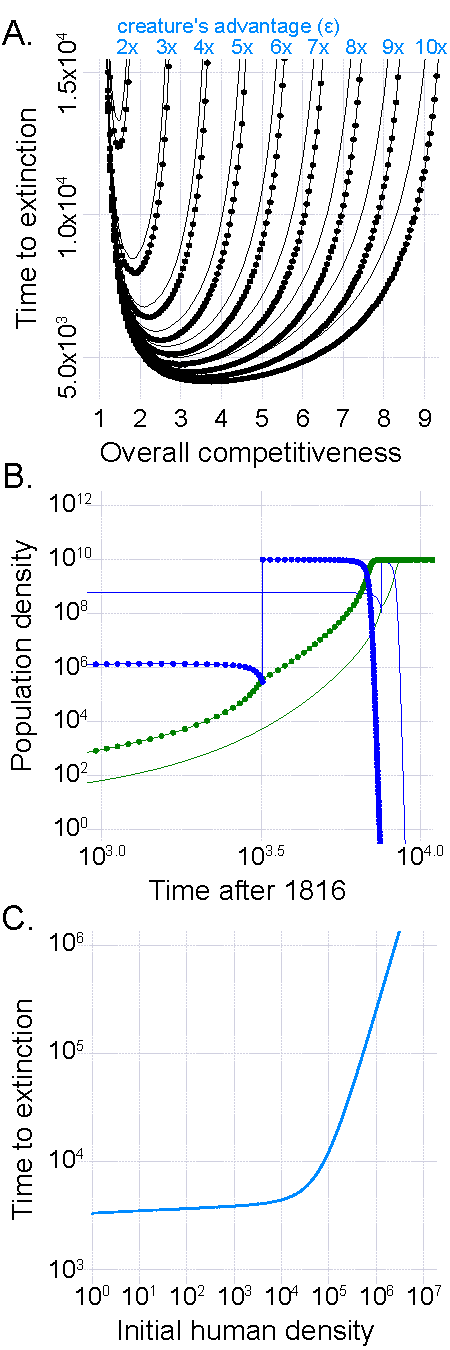
\includegraphics[width=0.25\textwidth]{fig_combined.pdf}
  \end{center}
  \vspace{-15pt}
  \caption{\footnotesize 
  A. Extinction time given competitive environment.
  B. Population trajectories for humans (blue) and creatures (green) given initial growth in the Amazon (dotted) and Europe (solid).
  C. Time to extinction vs. the human population size during initial growth of the creature population.
  }
  \vspace{2pt}
    \label{fig}
\end{wrapfigure}
When the overall level of competition is very low, the time to extinction is effectivity infinite, meaning that creatures and humans effectively coexist (Fig. 1A).
As the overall level of competition increases, we our model shows that the time to extinction drops precipitously to a minimum and then increases, and this becomes more exaggerated as the creature's competitive advantage increases.
Intriguingly, if the overall level of competition is very high, despite the creature's competitive advantage, they are doomed to extinction, such that the time to human extinction is also infinite.
This result occurs because the creature population begins at $n=2$ individuals, while human populations are much higher, and this asymmetry prevents the creature population from gaining a foothold under severe competitive pressures.
The global model reveals that the worst case scenario ($a_hm=xx,\epsilon=xx$) time to human extinction is $t_e = XXXX$.

Given the asymmetry in the initial size of the human vs. creature populations, it may be the case that the competitive environment in which the two \emph{begin} to interact is important.
The creature tells Frankenstein ``\emph{I will go to the vast wilds of South America}'', and this appears to be a conciliatory gesture.
How does the relocation of the creature and its companion to the Amazon alter projected extinction times?
We can address this question by assessing human extinction time if the creature first relocates to the Amazon (dotted curves, Fig. 1A,B) compared to a scenario where creatures immediately compete with the 1816 European populace (solid curves, Fig. 1A,B).

If we assume that the creature population (green dotted line, Fig. 1B) only begins to compete globally after it surpasses the Amazonian human population (blue dotted line, Fig. 1B -- the vertical jump denotes the transition from competing within the Amazon to competing globally), we find that the extinction time is less than if the creatures (green solid line, Fig. 1B) immediately begin competing  with the much larger European populace (blue solid line, Figure 1B) followed by the global population.
This $t_e$ for the Amazonian scenario holds across all levels of competition and for all values of $\epsilon$ (Fig. 1A).
The low-human-density Amazon thus serves as a catalyst for accelerating the creature's initial population growth, thus decreasing the time to human extinction, compared to the slower dynamics that occur when the small creature population must immediately compete with the dense 1816 European populace.
Low-density catalysts that act on the initial growth of an invading organism generally lowers the time to extinction of the resident population (Fig. 1C).
Indeed, the creature's concession to escape to the wilds of South America may have been a worst-case scenario, motivating Frankenstein to destroy the creature's companion, and eventually leading to the deaths of those he loved as well as his own.

%In Europe, XXXX years elapse before the creature population (green solid lines, Fig. 1B) overtakes humans (blue solid lines, Fig. 1B), and an additional XXXX years for it to drive humans extinct (we note that humans are assumed to have reached global carrying capacity by the time the creature population can compete globally). 
%If the creatures begins reproducing in the Amazon, XXXX elapse before the Amazon is overtaken, with another XXXX years before the global population of humans are driven extinct.

%The general conclusion -- invading via a catalyst
We have shown with a simple model that the initial population growth of an invading organism (the creature) within a low-density -- and by extension low-competitive environment -- can catalyze the invader's success, lowering the timescale of invasion to the exclusion of a resident species (humans).
Many invading species in ecological systems have competitive advantages over residents, as does the creature in the Frankenstein story, such that even small competitive effects on the resident can lead to extinction over ecological timescales (Fig. 1A).
The decision that Frankenstein makes, at the cost of his own destruction, was thus a prescient one, demonstrating that Shelley had an implicit understanding of the dynamics and potential horrors of niche overlap and competitive exclusion of invading species.
These issues are pertinent to our own world, which is now replete with \emph{creatures}:
those left to invade after native environments are destroyed or fragmented,
those that are distributed across the world by global transportation networks,
and those that are created or modified to suite our own needs.
In the bicentennial of Mary Shelley's Frankenstein, perhaps there is no better time to reconsider Frankenstein's creation and the horrors of competitive exclusion.




\end{document}














